\documentclass[]{article}

\usepackage[letterpaper, portrait, margin=1in]{geometry}
\usepackage{graphicx}

\interfootnotelinepenalty=10000

\title{Continuous Annotation Fusion via Rank-based Signal Warping}
\author{Brandon Booth}

\begin{document}

\maketitle

\section{Introduction}
Annotation fusion has been studied a lot (cite?).  Modern methods for fusing continuous annotations attempt to correct for known artifacts.  Some methods attempt to correct for lag in reaction time to changes in the stimulus.  These methods range from simple shifts in time to dynamic time warping where varying-length time windows are shifted different amounts of time.  These approaches require some representation of the target stimulus and often use several features extracted from the stimulus for time alignment.  The obvious down side to these approaches is that the alignment may fail if changes in the extracted features to not correspond to perceivable changes in the stimulus.

Other fusion methods model the different kinds of artifacts introduced by different types of annotators (cite Rahul).

Other fusion methods use event detection to locate points of interest in time and use windows between these boundaries for fusion (maybe? cite?).

The problems for which modern fusion approaches are adapted are primarily hidden state estimation problems such as the engagement level of a student viewing an online lecture.  Because for these types of problems the true value of the hidden state is not known, fusion approaches are typically validated using the resulting fused signal in a machine learning context to show that the model is better able to predict the target.  The problem with this type of validation is that it conflates any potential success of the fusion approach with the success of the learning model making it difficult to tell whether the fusion approach actually leads to a better representation of the object truth signal (e.g. the actual engagement value of a student).  To this end, we conduct our own study where annotators are instructed to provide continuous annotations in real-time where an objective truth signal is known a priori.  We are careful to pick a task where differences in each annotator's prior biases and perception lead to disagreements and artifacts in each annotation signal.

\section{Experiment and Results}
Ten annotators were asked to annotate the level of ``green-ness'' in a video.  The video was 4:27 minutes in length, 864x480 resolution, and comprised entirely of solid color frames of green at varying green channel values in RGB color space.  The green value was designed to change both slowly and rapidly at different times and frequencies and also in an unpredictable manner, but did not contain any sudden oscillations.  The slow varying and smooth changes were chosen because they mimic the often slow changes in other hidden mental state problems (engagement, productivity, etc. (cite?)).  Avoiding sudden oscillations means the annotators were not required to make any ``twitch'' reactions during the annotation process which would have added unnecessary artifacts.

The annotation process occurred in real time.  A slider widget representing a float value between zero and one was displayed and annotators used a mouse to move the slider as they watched the video.  The value of the slider was recorded for each video frame.  Figure \ref{fig:annotation_ui} shows the interface.

\begin{figure}
	\centering
	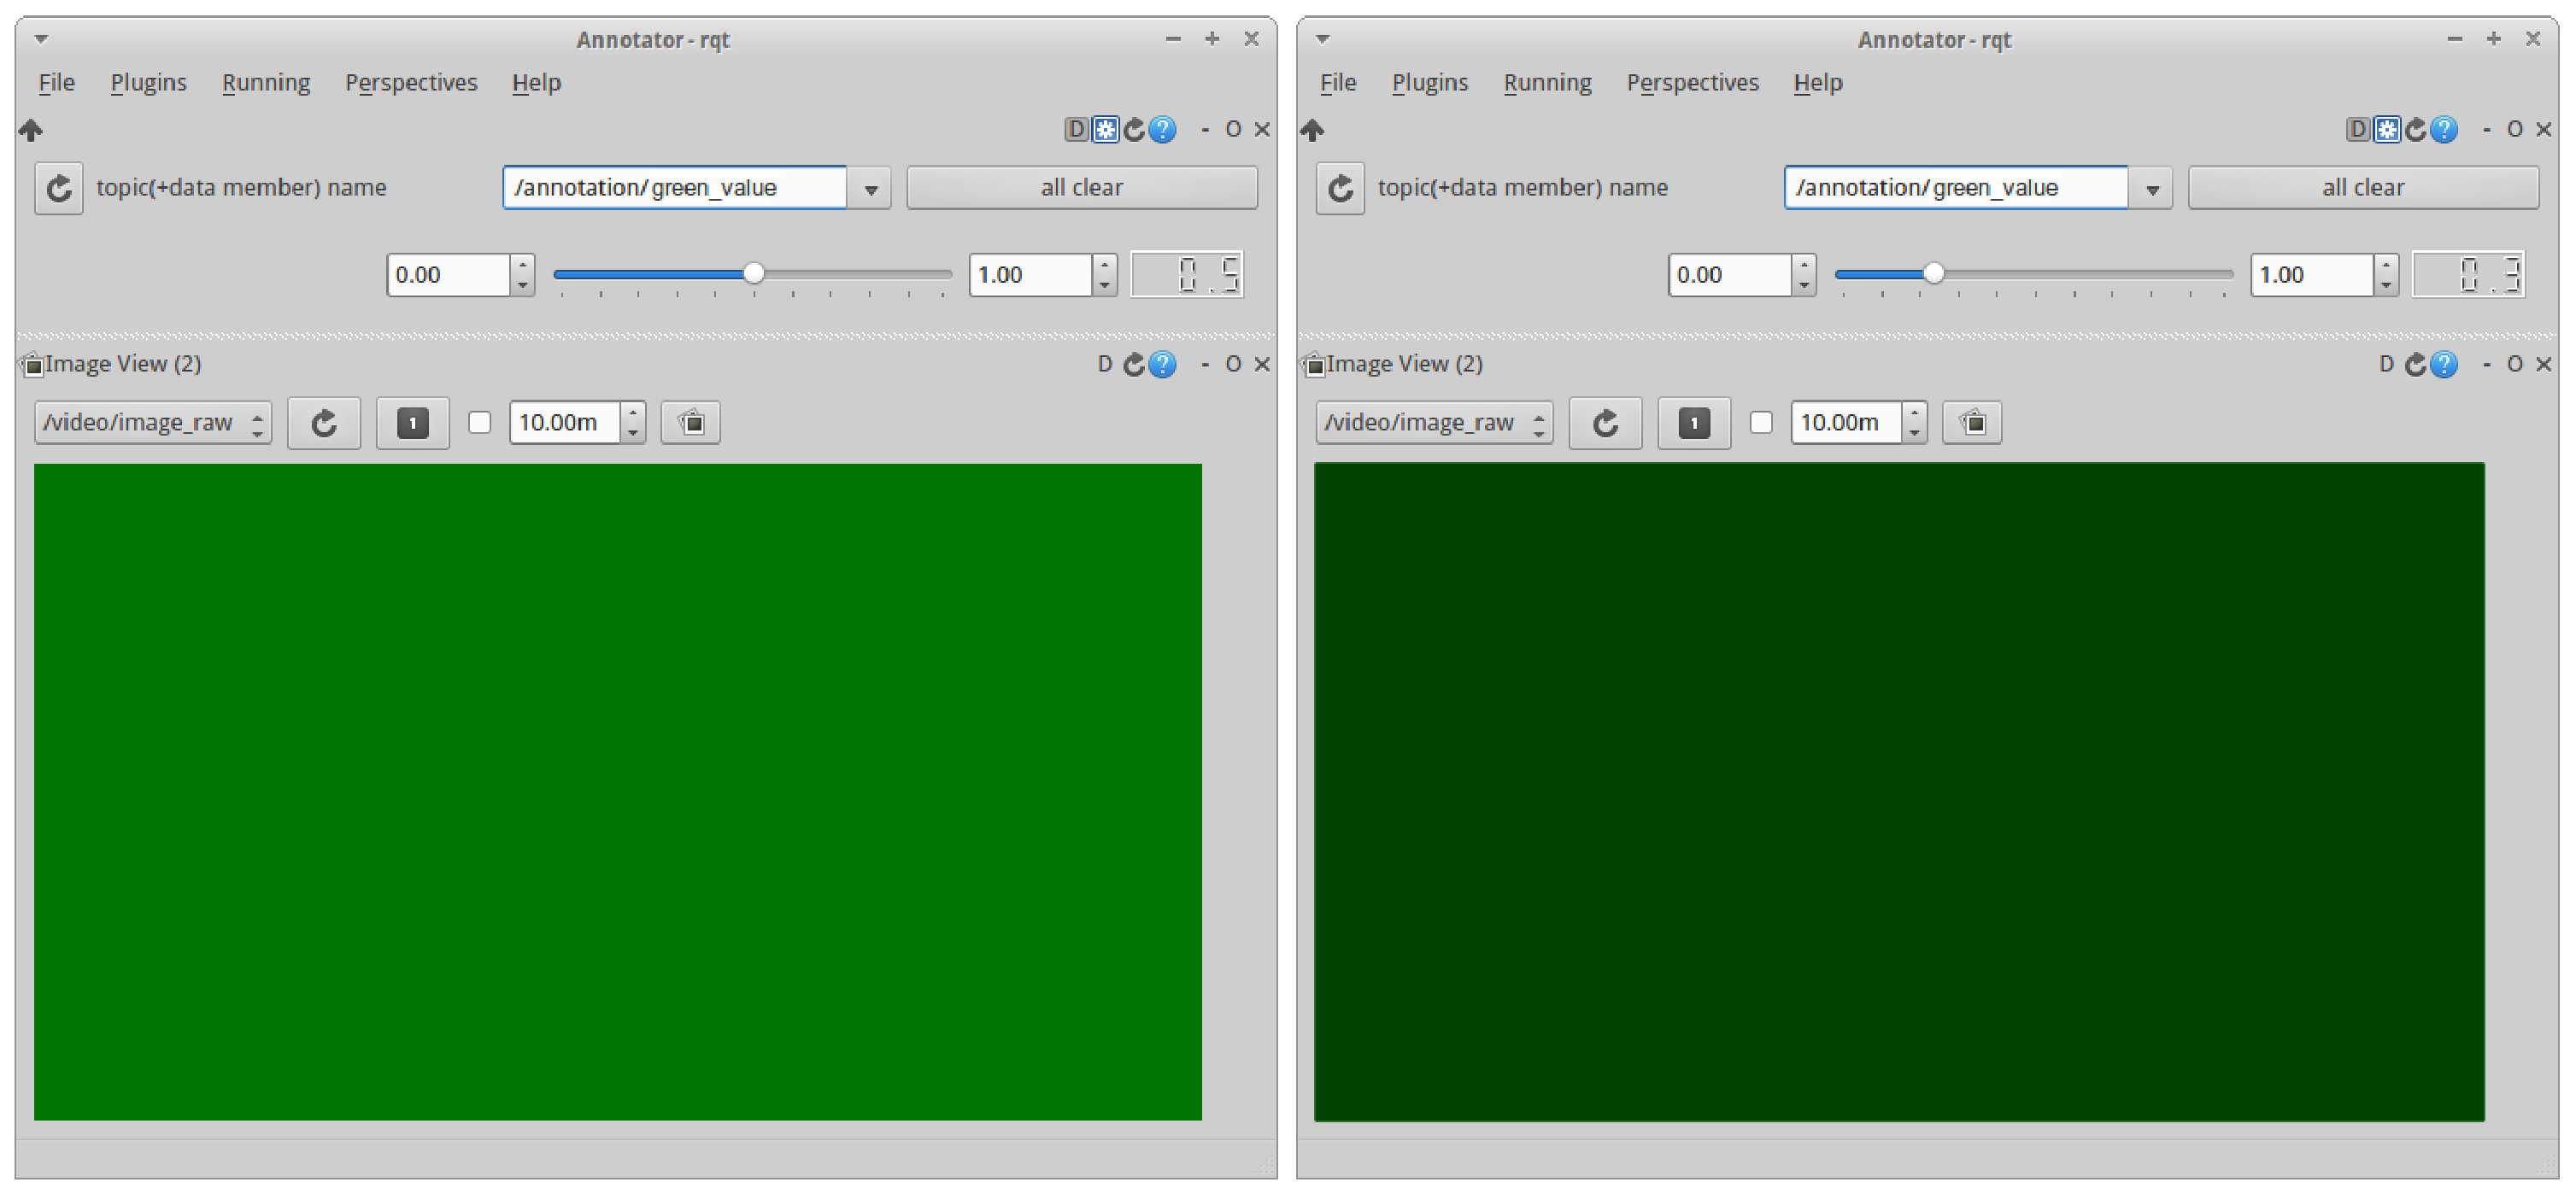
\includegraphics[width=0.8\textwidth]{images/green_ui}
	\caption{Snapshot of the user interface for the green channel value annotation task}
	\label{fig:annotation_ui}
\end{figure}

Figure \ref{fig:annotations_ot} shows a plot of all ten annotations alongside the objective truth.  This plot suggests that annotators are generally quite good at capturing large changes and trends for this task, but have difficulties in several areas.  First, most annotations tend to over shoot the target value when annotating increases or decreases in value over a period of time.  This is perhaps due to the lack of a reference color for various values of green thereby forcing annotators to estimate rate of change and focus on annotating a consistent rise or fall in the value.  By this logic, we consider the tendency to overestimate rather than underestimate merely a coincidence in this example, though it may be illustrative of a psychological trend.  Secondly, we note that approximately half of the annotators struggle to capture the lack of change in the stimulus especially near the 100 to 150 second time interval.  We posit this artifact is mainly due to the annotators having a few moments to stop focusing on capturing the value changes and refocus on accuracy.  In these cases it seems the annotators noticed the value of the slider did not match their perception of the green value and thus changed the slider value to attempt to move it to the correct location.  Lastly, we note that similar green values are annotated inconsistently over time.  In particular, there is a significant difference in average annotation value per annotator between the sections where the stimulus is at a 0.5 constant value.

This last observation suggests that even for this relatively simple annotation task, it is difficult for annotators to accurately capture the trends while preserving self-consistency over time.  It seems reasonable to conclude that annotators are more focused, and perhaps even better at, faithfully capturing trends and less able to accurately assess the true value at any point in time.  Our primary aim in this paper is to propose a procedure to correct for these global inconsistencies and artifacts.

\begin{figure}
	\centering
	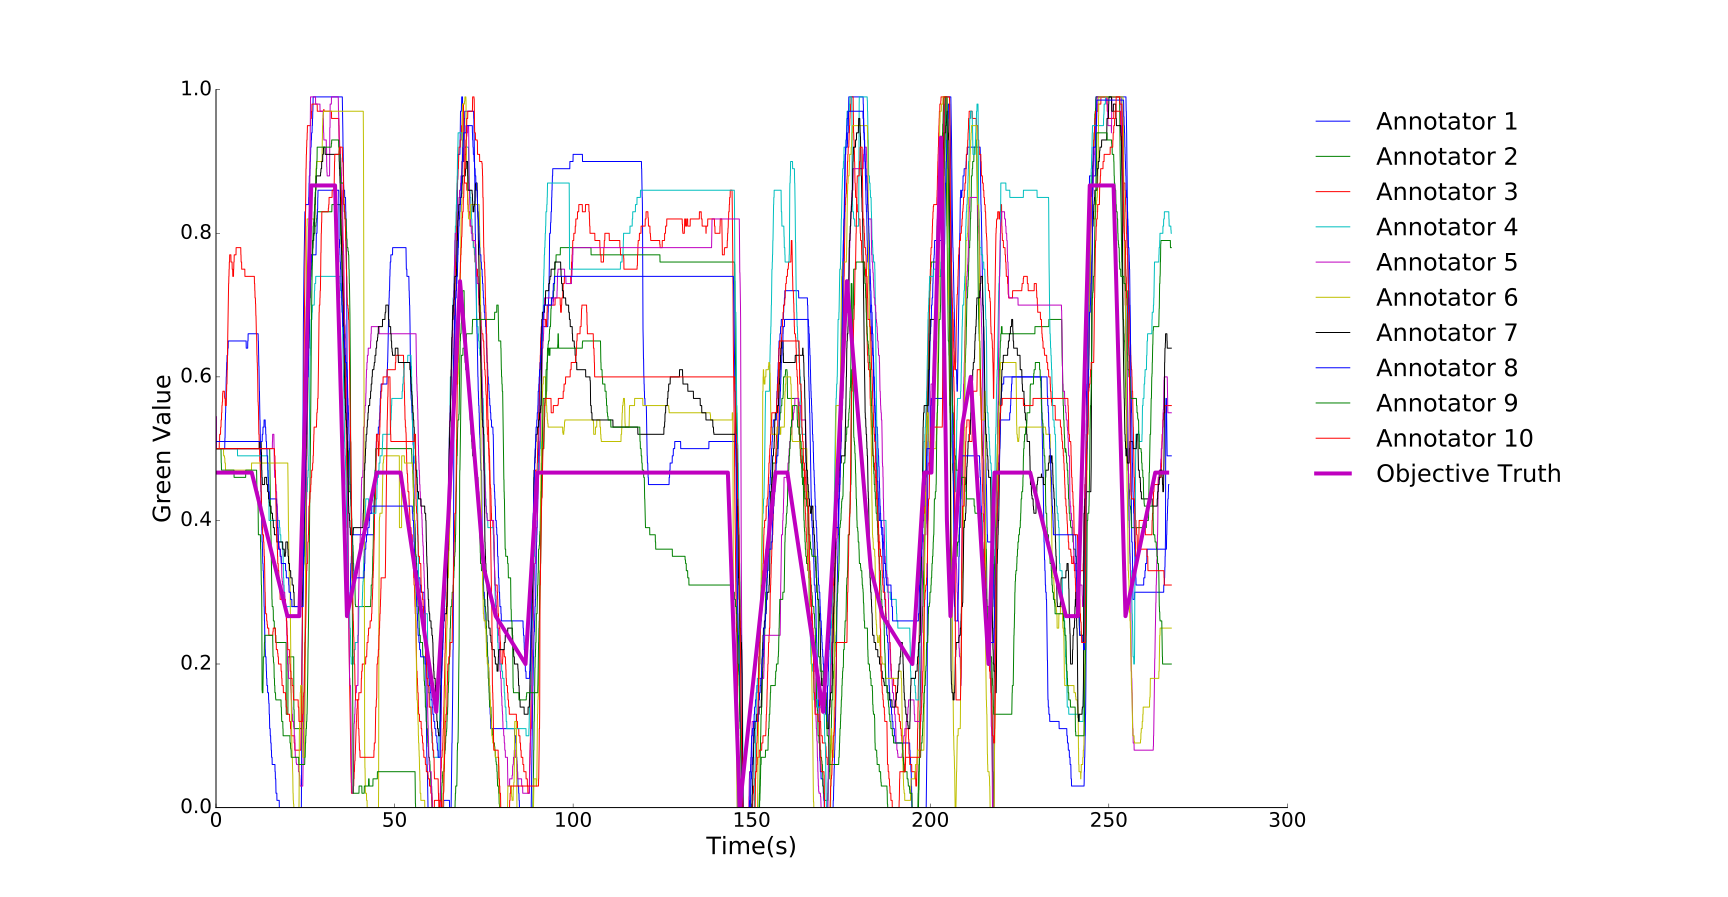
\includegraphics[width=1.0\textwidth]{images/annotations_ot}
	\caption{Annotations of green channel values in the video alongside the true value}
	\label{fig:annotations_ot}
\end{figure}

\section{Ground Truth Estimation}

We present a method for annotation fusion for the purposes of establishing a ground truth signal that corrects for global inconsistencies, artifacts, and errors introduced during the real-time continuous annotation process.  The following list names each step of the procedure.

\begin{enumerate}
	\item Annotation average
	\item Total variation denoising (TV denoising)
	\item Constant interval extraction
	\item Triplet
	\item Non-metric multi-dimensional scaling (NMDS)
	\item Signal warping
\end{enumerate}

The first step averages all annotations to limit the influence of systemic noise such as mouse jitter and sampling aliasing.  Total variation (TV) denoising is used to approximate the average signal as a piecewise-constant step function.  Nearly constant intervals are extracted from the denoised signal and correspond to time spans where annotators generally agree that the hidden objective truth did not change noticeably.  At this point, we focus our efforts to fix-up the signal by asking for additional information from the annotators to help re-evaluate the proper order of the target with respect to the stimulus during these time intervals.  We collect ordinal relationships between triplets of these constant intervals from annotators and employ a 2D ordinal embedding technique to re-rank the intervals.  Finally, the original average signal is warped linearly to more closely match the re-ranked piecewise-constant step function.  Each of these steps and their assumptions are described in detail in the corresponding section below.

\subsection{Total Variation Denoising}
Total variation denoising has been successfully used to remove granular noise from images while simultaneously preserving signal edges.  Our aim at this step of the procedure is to identify regions in the average annotation signal where the stimulus is not changing noticeably.  We focus on obtaining a set of these time intervals under the assumption that annotators already capture the changes in the stimulus quite well and we only need to make adjustments to the constant portions.  TV denoising is preferable to other smoothing processes both because it explicitly attempts to model the function as a piecewise-constant step function as is desired, and also because it minimizes smoothing near transition boundaries which maximizes the size of each constant interval.

We use the Matlab TFOCS library to find a new signal $y_t$ that approximates the signal $x_t$ and minimizes:

\[
\min_{y_t} \Big[\sum_{t} (x_t - y_t)^2 + \lambda\sum_{t} |y_{t+1} - y_{t}|\Big]
\]

The parameter $\lambda$ controls the influence of the temporal variation term and encourages signals that look more piecewise-constant.  In general this parameter needs to be tuned to produce a desirable TV signal.  For this study, we casually hand-tuned $\lambda$ and settled on a value of 0.05.  Figure \ref{fig:average_and_objective} shows the averaged annotation signal and the TV denoised signal.

\begin{figure}
	\centering
	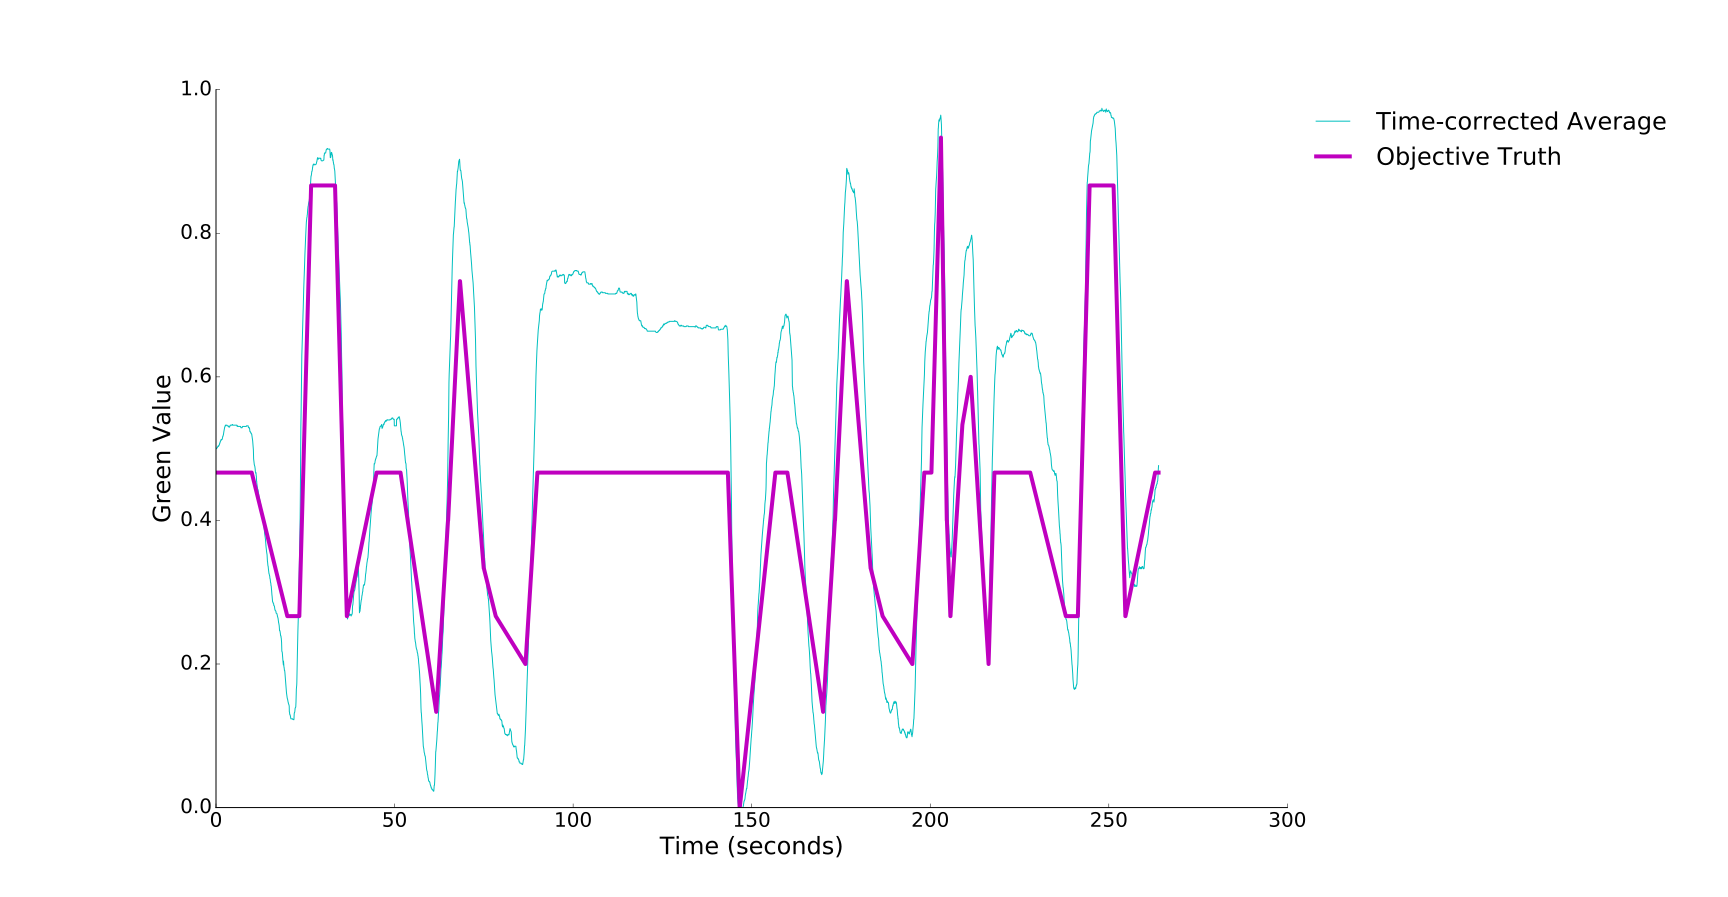
\includegraphics[width=0.49\textwidth]{images/average_and_objective}
	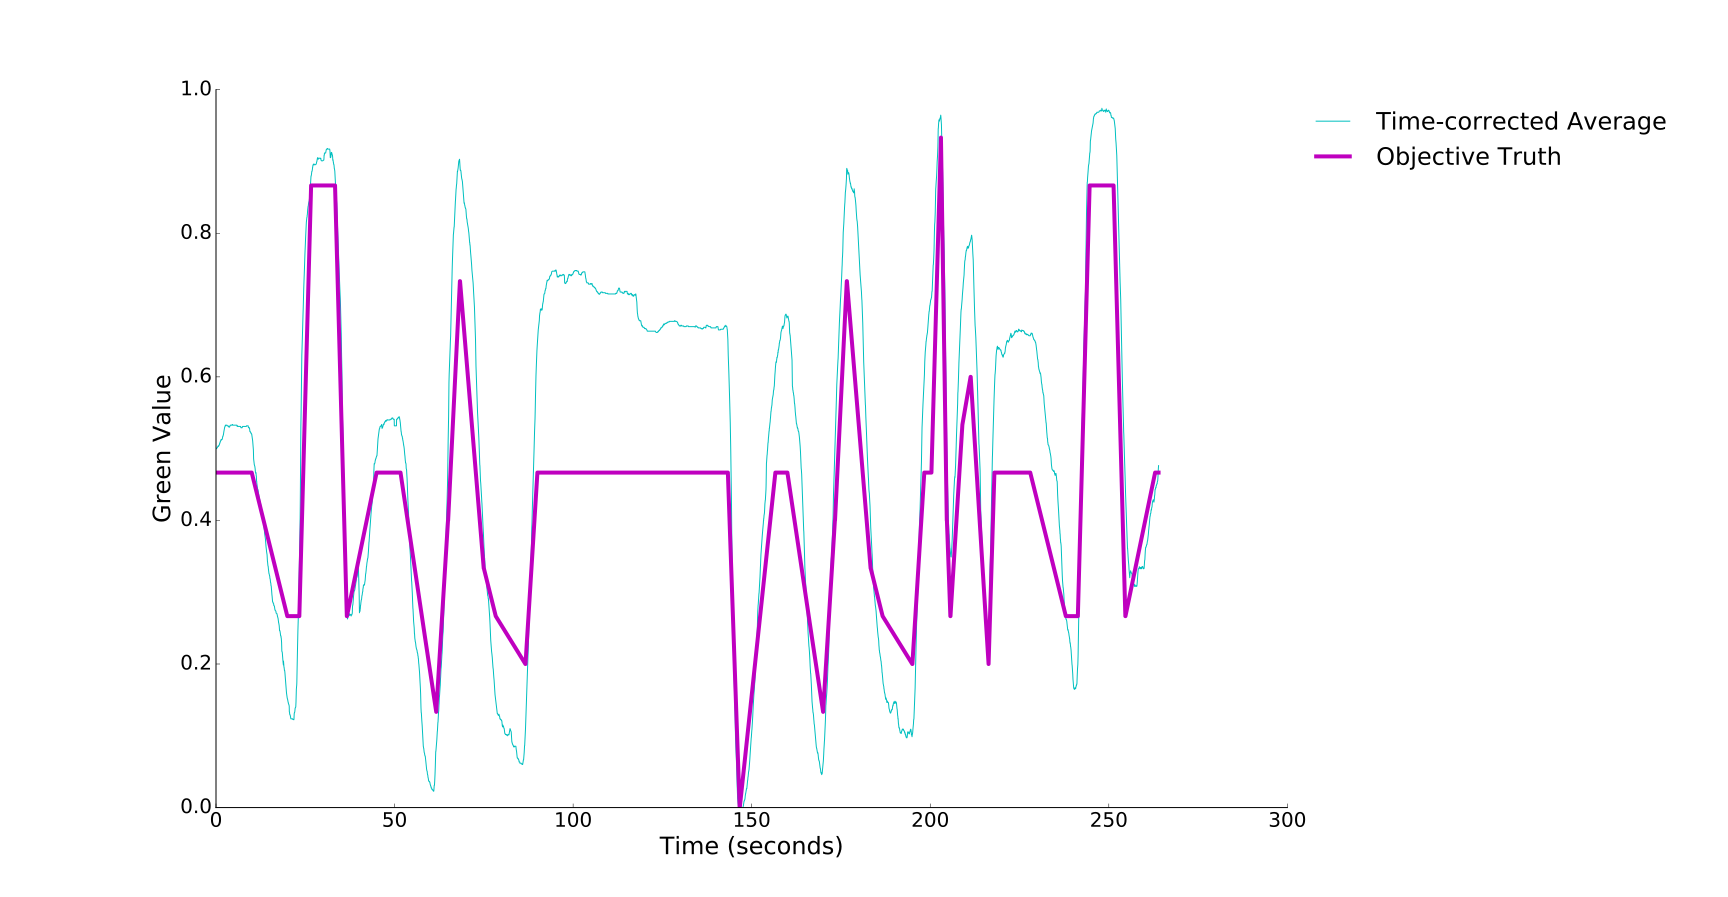
\includegraphics[width=0.49\textwidth]{images/average_and_objective}
	\caption{Plot of annotation average and objective truth on the left and TV denoised average signal with extracted constant intervals on the right}
	\label{fig:average_and_objective}
\end{figure}

\subsection{NMDS}
\subsection{Signal Warping}
\section{Results}
Show correlations chart with perfect information

Show results with imperfect information (incomplete triplets)

Show results with conflicting triplets and complete information

Show results with missing information and incomplete triplets (simulation of adversarial annotator, ISN'T THIS THE BYZANTINE GENERALS PROBLEM?)

\section{Discussion}
Why is this better?  Even with perfect triplet comparison information there is no way for NMDS to reconstruct the scale.  NMDS does guarantee that there exists some monotonic transformation of the output that would yield the original signal.  If the goal is to treat the warped signal as a ground truth and then machine learn with it, then there is no need to learn this monotonic transformation function because the ``distorted'' ground truth signal is still self-consistent (i.e. the warped signal is approximately a dilation of the true signal).

\section{Conclusion}

\section{Future Work}
Finding the right value for the tunable TV denoising constant.  Perhaps choosing a parameter that creates N constant intervals where concentration bounds guarantee fewer than M type I/II errors given X annotators and P probability of adversarial ordinal comparisons.

Adjusting the window size for the constant interval extraction and the maximum allowable slope for the nearly constant portions.



\bibliography{references}
\bibliographystyle{ieeetr}

\end{document}